%!TeX root=../tese.tex
%("dica" para o editor de texto: este arquivo é parte de um documento maior)
% para saber mais: https://tex.stackexchange.com/q/78101/183146

%% ------------------------------------------------------------------------- %%
\chapter{Árvores splay}
\label{cap:arvores-splay}

\newtheorem{caso}{Caso}

Neste capítulo apresentaremos as árvores splay, desenvolvidas por \cite{selfadjustingbst}. As árvores splay são uma ABB que, além das rotinas usuais de busca, inserção e remoção, possuem uma rotina extra, chamada splay. Essa rotina deve ser acionada ao final de cada operação feita numa árvore splay, aplicada ao nó mais profundo que foi visitado durante a operação Descreveremos o funcionamento da operação splay, analisaremos o custo amortizado de operações em árvores splay e introduziremos a Conjectura da Otimalidade Dinâmica.


\section{Introdução}
A altura de uma árvore binária de busca é o comprimento de um caminho mais longo da raiz da árvore a uma de suas folhas. É sabido que a altura de uma ABB com $n$ nós é um valor entre $\log_2 n$ e $n-1$. O pior caso das operações de busca, inserção, remoção e outros em árvores binárias de busca é exatamente a altura da árvore. Por isso, surgiram na literatura várias propostas de implementações de ABBs que mantém alguma propriedade que implica que a altura da árvore se mantém logarítmica no número de nós da ABB. Tais implementações, em geral, carregam informação extra nos nós da árvore e executam rotações durante as inserções e remoções porém não alteram a árvore durante as buscas.

Uma alternativa a essas estratégias é a árvore splay. Árvore Splay é uma árvore binária de busca balanceada proposta por \cite{selfadjustingbst}. Diferentemente das árvores binárias balanceadas citadas anteriormente, a árvore splay se reestrutura após qualquer operação, inclusive após as buscas e não utiliza armazenamento adicional.

% ESTÁ RUIM!
A árvore splay é uma ABB que segue a heurística “move to front”, ou seja, a ideia central é que a medida que operações são realizadas na estrutura, os elementos são movidos para perto da raiz de uma maneira particular com intuito de manter na raiz o nó que guarda a última chave acessada.
Com a tendência dos nós com chave mais recentemente acessadas estarem próximos da raiz, o custo de sequências de acessos repetitivos tende a diminuir e essas reestruturações também auxiliam a árvore splay a dispor seus nós de maneira mais balanceada, reduzindo a altura total da árvore em alguns casos.

%Mostre o código da busca com a chamada à rotina splay
%Mostre o código do splay

{
    \tikzset{
        nodes = {draw, circle, minimum size = 8mm},
        edge from parent path = {(\tikzparentnode) -- (\tikzchildnode)},
    sibling distance=20pt,
    n/.style = {draw=none},
    r/.style = {fill=white},
    b/.style = {fill=gray},
    edge from parent/.append style={-, shorten >= 0, shorten <= 0}
    }

\section{Operação Splay}

A essência da árvore splay está na operação splay. A operação splay é a responsável por mover um nó específico para a raiz por meio de sucessivas rotações duplas. Essa operação é fundamental para o funcionamento da estrutura e é utilizada por todas as outras operações.

A operação splay se utiliza de três tipos distintos de rotações para trazer um nó para a raiz: zig, zig-zig e zig-zag.

Seja $x$ o nó que a operação splay está deslocando para a raiz. 

\subsection{Caso zig}

A rotação zig acontece quando $x$ é descendente direto do nó raiz. Neste caso apenas é necessário realizar uma rotação no nó $x$ e $x$ se encontrará na raiz da árvore. Este é o único de rotação única.

Como a operação splay se encerra quando o nó analisado chega a raiz, esta rotação é executada no máximo uma vez durante a execução desta operação. Ela só acontece quando o caminho de $x$ até a raiz da ABB tem comprimento ímpar.

\begin{figure}[h]
    \centering
    \begin{comment}
    \begin{tikzpicture}[
        ed/.style = {densely dashed, shorten >= 5pt},
        alpha/.style = {regular polygon, regular polygon sides=3, draw, minimum size=1.1cm, inner sep=2pt, anchor=south},
        circ/.style = {draw, shape=circle, inner sep=2pt, anchor=south},
        level distance=1.5cm,
        sibling distance=0.5cm
        ]
        
        \begin{scope}[local bounding box=scope1]
        \Tree [.$y$ [.$x$ \node[alpha]{a}; \node[alpha]{b}; ] \node[alpha]{c}; ]
        \end{scope}
        
        \begin{scope}[xshift=6cm, local bounding box=scope2]
        \Tree [.$x$ \node[alpha]{a}; [.$y$ \node[alpha]{b}; \node[alpha]{c}; ] ]
        \end{scope}
        
        \draw[->] ([yshift=-0.5*\ht\strutbox,xshift=0.5cm]scope1.east) -- node [n] {} ([yshift=-0.5*\ht\strutbox,xshift=-0.5cm]scope2.west); % Ajusta a flecha centralizada
        
        \draw[->] ([yshift=-1.65cm, xshift=-0.285cm]scope1.north) arc (180:0:0.7cm);
        
    \end{tikzpicture}
    \end{comment}
    \includegraphics{imagens/zig.pdf}
    \label{fig:zig}

\caption{Caso zig com $x$ nó esquerdo da raiz.}
\end{figure}

\subsection{Caso zig-zig}

A rotação zig-zig é realizada quando $x$ e seu pai possuem a mesma orientação em relação aos seus pais, ou seja, ambos são filhos direitos ou ambos são filhos esquerdos. Neste caso, é necessário rotacionar o pai de $x$ primeiro e em seguida rotacionar $x$.

\begin{figure}[H]
    \centering
    \begin{comment}
    \begin{tikzpicture}[
        ed/.style = {densely dashed, shorten >= 5pt},
        alpha/.style = {regular polygon, regular polygon sides=3, draw, minimum size=1.1cm, inner sep=2pt, anchor=south},
        level distance=1.5cm,
        sibling distance=0.25cm
        ]
        
        \begin{scope}[local bounding box=scope1]
        \Tree [.$z$  [.$y$ [.$x$ \node[alpha]{a}; \node[alpha]{b}; ] \node[alpha]{c};] \node[alpha]{d};]
        \end{scope}
        
        \begin{scope}[xshift=6cm, local bounding box=scope2]
        \Tree [.$x$ \node[alpha]{a}; [.$y$ \node[alpha]{b}; [.$z$ \node[alpha]{c}; \node[alpha]{d}; ]]]
        \end{scope}
        
        \draw[->] ([yshift=-0.5*\ht\strutbox,xshift=0.5cm]scope1.east) -- node [n] {} ([yshift=-0.5*\ht\strutbox,xshift=-0.5cm]scope2.west); % Ajusta a flecha centralizada
        
        \draw[->] ([yshift=-2.20cm, xshift=-0.98cm]scope1.north) arc (198:-18:0.7cm);
        \draw[->,red] ([yshift=-3.67cm, xshift=-1.89cm]scope1.north) arc (198:-18:0.7cm);
    
    \end{tikzpicture}
    \end{comment}
    \includegraphics[scale=0.9]{imagens/zigzig2.pdf}
    \label{fig:zigzig}
\caption{Caso zig-zig com $x$ e $y$ ambos filhos esquerdos.}
\end{figure}


\subsection{Caso zig-zag}

A rotação zig-zag é realizada quando $x$ e seu pai possuem orientação diferentes em relação aos seus pais, ou seja, $x$ é filho direito e o pai de $x$ é filho esquerdo ou $x$ é filho esquerdo e o pai de $x$ é filho direito. Neste caso, é necessário rotacionar $x$ duas vezes. Vale ressaltar que cada rotação será feita para um lado.

Note que esta rotação propositalmente diminui a altura da subárvore analisada.
    
\begin{figure}[H]
    \centering
    \begin{comment}
    \begin{tikzpicture}[
        ed/.style = {densely dashed, shorten >= 5pt},
        alpha/.style = {regular polygon, regular polygon sides=3, draw, minimum size=1.1cm, inner sep=2pt, anchor=south},
        level distance=1.5cm,
        sibling distance=0.25cm
        ]

        \begin{scope}[local bounding box=scope1]
            \Tree [.$z$  [.$y$ \node[alpha]{a}; [.$x$ \node[alpha]{b}; \node[alpha]{c}; ]] \node[alpha]{d};]
        \end{scope}
        
        \begin{scope}[xshift=6cm, local bounding box=scope2]
            \Tree [.$z$  [.$x$ [.$y$ \node[alpha]{a}; \node[alpha]{b}; ] \node[alpha]{c};] \node[alpha]{d};]
            \end{scope}
            
            \begin{scope}[xshift=12cm, local bounding box=scope3]
                \Tree [.$x$ [.$y$ \node[alpha]{a}; \node[alpha]{b};] [.$z$  \node[alpha]{c}; \node[alpha]{d};]]
            \end{scope}
                
            \draw[->] ([yshift=-0.5*\ht\strutbox,xshift=0.3cm]scope2.east) -- node [n] {} ([yshift=-0.5*\ht\strutbox,xshift=-0.3cm]scope3.west);
                
            \draw[->] ([yshift=-3.67cm, xshift=0.67cm]scope2.north) arc (-18:198:0.7cm);
                \draw[->,red] ([yshift=-3.69cm, xshift=-0.82cm]scope2.north) arc (198:-18:0.86cm);
                
    \end{tikzpicture}
    \end{comment}
    \includegraphics[scale=0.85]{imagens/zigzag2.pdf}
    \caption{Caso zig-zag com $x$ filho direito e $y$ filho esquerdo.}
\end{figure}
        
}

Uma série de operações podem ser implementadas nessas estruturas como inserção, remoção, busca, junção e divisão. Todas essas operações chamam a operação splay no nó mais profundo visitado durante sua execução. Para esse trabalho, o importante é saber que ao final de cada acesso, o nó com a chave acessada será levado para a raiz pela operação splay. Veja a execução de uma operação splay por completo na Figura~\ref{fig:fullsplay}.

\begin{figure}
    \includegraphics[scale=0.77]{imagens/fullsplay2.pdf}
    \caption{Execução da operação splay após acesso na chave 4.}
\label{fig:fullsplay}
\end{figure}

\section{Análise da operação splay}

Definimos o custo da operação splay como o número de rotações realizadas durante sua execução. Caso nenhum rotação seja realizada, definimos o custo dessa operação como 1. 

Faremos uma análise amortizada da estrutura. Seja $S$ a árvore splay sendo analisada, $c$ o custo real de uma operação splay e \( \hat{c}\) o custo amortizado de uma operação splay. Definimos $s(x)$ como o tamanho da subárvore enraizada no nó $x$. Definimos o potencial local do nó $x$ como $r(x) = \log_2(s(x))$. Por fim, definimos $\Phi$ como o potencial da árvore splay inteira que é a somatória do potencial local de todos os nós da árvore.

\begin{lemma}
    O custo amortizado de qualquer rotação da operação splay no nó $x$ é $< 3(r'(x) - r(x)) + 1$, onde $r$ é o potencial local antes da operação e $r'$ o potencial local depois da operação. $\Phi$ é o potencial da árvore antes da operação e $\Phi'$ o potencial da árvore depois da operação
\end{lemma}

\begin{proof}
    Denotemos por $y$ o nó pai de $x$ antes da rotação e por $z$ o pai de $y$ antes da operação, se $z$ existir.

    \textit{Caso zig}.   
    \begin{align*}
        \hat{c} &= c + \Delta \Phi,\\
        &= 1 + r'(x) + r'(y) - r(x) - r(y), \quad & \text{}\\
        &< 1 + r'(x) - r(x) \quad & \text{pois $r(y) > r'(y)$},\\
        &< 1 + 3(r'(x) - r(x)) \quad & \text{pois $r'(x) > r(x)$}.\\
    \end{align*}

    Para os próximos casos será essencial entender uma propriedade da função logaritmo. A função logaritmo é côncava, ou seja, $\frac{\log_2(a) + \log_2(b)}{2} \leq \log_2(\frac{a+b}{2})$. Isso pode ser evidenciado pela Figura~\ref{fig:log}.

    \begin{figure}
        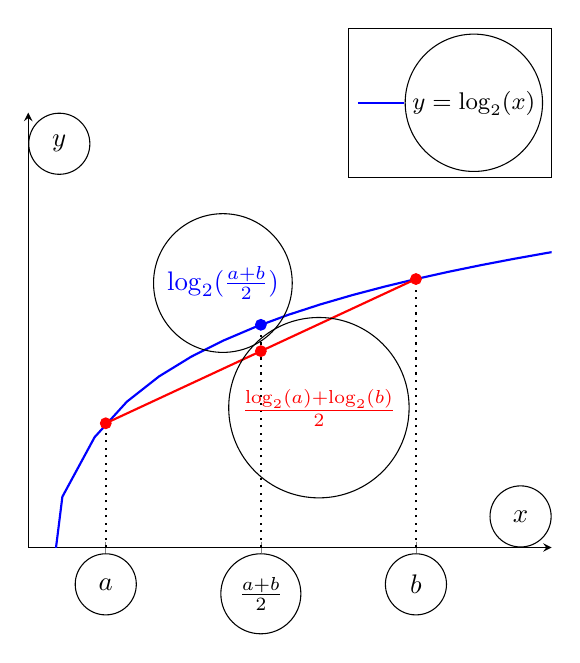
\begin{tikzpicture}[scale=0.97]
            \begin{axis}[
                axis lines = middle,
                xmin=0, xmax=27,
                ymin=0, ymax=7,
                xtick={4,12,20},
                xticklabels={$a$,$\frac{a+b}{2}$,$b$},
                ytick=\empty,
                xlabel = {$x$}, % Nome do eixo x
                ylabel = {$y$},
                legend style={
                    at={(1,0.85)},  % Move a legenda mais para baixo
                    anchor=south east,
                    font=\small   % Reduz o tamanho da fonte da legenda
                }
            ] % Função y = log2(x)
                \addplot[blue, thick, domain=0.1:40] {log2(x)};
                
                % Pontos
                \addplot[only marks, red] coordinates {(4,2)}; % Ponto A
                \addplot[only marks, red] coordinates {(20, 4.3219281)}; % Ponto B
                \addplot[only marks, blue] coordinates {(12,3.5849625)}; % Ponto C
                \addplot[only marks, red] coordinates {(12,3.16096405)}; % Ponto D
        
                % Reta entre A e B
                \addplot[red, thick] coordinates {(4,2) (20, 4.3219281)};
                
                % Linhas pontilhadas
                \draw[thick, dotted] (axis cs:4,0) -- (axis cs:4,2);   % Linha pontilhada de A
                \draw[thick, dotted] (axis cs:20,0) -- (axis cs:20, 4.3219281);   % Linha pontilhada de B
                \draw[thick, dotted] (axis cs:12,0) -- (axis cs:12, 3.5849625);
                
                % Nomes dos pontos
                \node at (axis cs:12, 3.5849625) [anchor=south east, text = blue, xshift=0.15cm, yshift=-0.1cm] {$\log_2(\frac{a+b}{2})$};  % Nome do ponto C
                \node at (axis cs:12, 3.16096405) [anchor=north west, text=red, xshift=-0.08cm, yshift=0.1cm] {$\frac{\log_2(a) + \log_2(b)}{2}$};  % Nome do ponto D
                
                % Legenda
                \addlegendentry{$y = \log_2(x)$} % Legenda para a função
            \end{axis}
        \end{tikzpicture}
    \caption{Na imagem estão destacados pontos $a$ e $b$ arbitrários na função. Como a função é côncava, o ponto com $y = \frac{\log_2(a) + \log_2(b)}{2}$ nunca estará acima do ponto com $y = \log_2(\frac{a+b}{2})$.}
    \label{fig:log}
    \end{figure}
    
    \textit{Caso zig-zig}.   
    \begin{align*}
        %\hat{c} &= c + \Delta \Phi, & \hspace*{-1.2cm} \text{amortizado = custo + diferença de potencial}, \\
        \hat{c} &= c + \Delta \Phi,\\
        &= 2 + r'(x) + r'(y) + r'(z) - r(x) - r(y) - r(z), \quad & \text{}\\
        &= 2 + r'(y) + r'(z) - r(x) - r(y) \quad & \text{pois $r'(x) = r(z)$},\\
        &< 2 + r'(y) + r'(z) - 2r(x) \quad & \text{pois $r(y) > r(x)$}, \\
        &< 2 + r'(x) + r'(z) - 2r(x) \quad & \text{pois $r'(x) > r'(y)$}.
    \end{align*}
    Por conta da propriedade da função $\log_2$ vista acima, temos que:
    \begin{align*}
        %\hat{c} &= c + \Delta \Phi, & \hspace*{-1.2cm} \text{amortizado = custo + diferença de potencial}, \\
        r(x) + r'(z) &= \log_2(s(x)) + \log_2(s'(z)), \quad & \text{}\\
        &= 2 \cdot \frac{\log_2(s(x)) + \log_2(s'(z))}{2}, \quad & \text{} \\
        &\leq 2 \log_2(\frac{s(x) + s'(z)}{2}) \quad & \text{propriedade de $\log_2$}, \\
        &< 2 \log_2(\frac{s'(x)}{2}) \quad & \text{pois $s'(x) > s(x) + s'(z)$}, \\
        &= 2 (\log_2(s'(x)) - \log_2(2)) \quad & \text{propriedade de $\log_2$}, \\
        &= 2 (r'(x) - 1).
    \end{align*}
    Assim, retornando ao problema original,
    \begin{align*}
        \hat{c} &< 2 + r'(x) + r'(z) - 2r(x), \\
        &< 2 + r'(x) +  2 (r'(x) - 1) - r(x) - 2r(x), \\
        &= 3(r'(x) - r(x)). \\
    \end{align*}
    \textit{Caso zig-zag}.   
    \begin{align*}
        %\hat{c} &= c + \Delta \Phi, & \hspace*{-1.2cm} \text{amortizado = custo + diferença de potencial}, \\
        \hat{c} &= c + \Delta \Phi,\\
        &= 2 + r'(x) + r'(y) + r'(z) - r(x) - r(y) - r(z), \quad & \text{}\\
        &= 2 + r'(y) + r'(z) - r(x) - r(y) \quad & \text{pois $r'(x) = r(z)$},\\
        &< 2 + r'(y) + r'(z) - 2r(x) \quad & \text{pois $r(x) < r(y)$},\\
        &< 2 + r'(x) - 2r(x) \quad & \text{pois $r'(y) + r'(z) < r'(x)$},\\
        &< 3(r'(x) - r(x)). \\
    \end{align*}
\end{proof}

\begin{theorem}
    O custo amortizado da operação splay é \( \mathcal{O}(\log n) \).
\end{theorem}

\begin{proof}
    O custo amortizado da operação splay no nó $x$ é a soma dos custos amortizados das rotações realizadas durante a operação.

    Denotemos por $\hat{c}_{\textit{splay}}$ o custo amortizado da operação splay e por $\hat{c}_{\textit{rotação}}$($i$) o custo amortizado da rotação $i$. Denotemos por $n$ o número de rotações realizadas por essa operação splay.
    \begin{align*}
        \hat{c}_{\textit{splay}} &= \sum_{i = 1}^{n} \hat{c}_{\textit{rotação}}(i), \\
        &< \sum_{i = 1}^{n} {3(r^{i+1}(x) - r^{i}(x)) + 1}, \\
        &= 3(r^{n+1}(x) - r^{1}(x)) + 1, \\ 
        &\leq 3\log_2n + 1 \quad & \text{pois $r^{n+1}(x) = \log_2(n)$}, \\ 
        &= \mathcal{O}(\log n).
    \end{align*}
\end{proof}


\section{Conjectura da Otimalidade Dinâmica}

Uma ABB online é \textit{dinamicamente ótima} se, para todas as sequências $X$, seu algoritmo de busca tem custo $\mathcal{O}(\textit{OPT(X)})$. De maneira mais geral, uma ABB online é \textit{$c$-competitiva} se executa todas as sequências $X$ suficientemente longas com custo no máximo $c$\,$OPT(X)$.

\cite{selfadjustingbst} conjecturaram que a árvore splay é dinamicamente ótima. Essa conjectura é conhecida por Conjectura da Otimalidade Dinâmica. Diversos pesquisadores já investigaram essa conjectura mas ainda pouco se sabe sobre ela. Os resultados obtidos com essas décadas de pesquisa não obtiveram sucesso provando ou refutando essa hipótese, porém provou-se que a árvore splay é uma estrutura que possui uma serie de propriedades que o $OPT$ também tem. 

Pouco se sabe sobre o $OPT(X)$ para uma sequência de acessos $X$. No próximo capítulo abordaremos a visão geométrica de buscas e em seguida buscaremos entender quais são as características do $OPT(X)$ dentro dessa nova abordagem. 